\chapter[Capítulo 6. Experimentos]{Experimentos}

Tras el análisis introductorio al contexto en el que nos situamos para hacer conocer al lector las técnicas que hay detrás del problema que queremos resolver y después de exponer y analizar la propuesta de trabajo a la que nos enfrentamos, entramos de lleno en la exposición del marco de trabajo en el que nos situaremos con los algoritmos que vamos a manejar, así como la muestra de resultados obtenidos en cuanto a comparativas realizadas y, por último, su posterior análisis, con el fin de concretar el éxito o fracaso de la teoría expuesta en capítulos anteriores.

\section{Marco de trabajo}

En esta sección, tal como hemos comentado, situaremos el marco de trabajo de nuestro experimento, formado por los conjuntos de datos que trataremos para este, junto con las medidas de precisión y monotonía que usaremos con los algoritmos con el fin de poder ser comparados por igual.

\subsection{Conjuntos de datos}

Primeramente comentaremos los conjuntos de datos a tratar con el fin de entender a que se enfrentarán nuestros algoritmos. Antes que nada cabe destacar que los data sets que vamos a utilizar son estáticos, es decir, no son datos que nos llegan en flujo (que es uno de los aspectos que queremos tratar en este documento), por tanto a la hora de realizar los experimentos habremos de simular la entrada de datos por un flujo en lugar de leerlos de forma directa. Los datos han sido sacados de \cite{ref16}



\begin{table}[]
	\begin{tabular}{|l|l|l|l|l|l|l|}
		\hline
		Data set & Instancias & Atributos & Numéricos & Nominales & Clases & NMI   \\ \hline
		ERA      & 1000       & 4         & 4         & 0         & 9      & 0.016 \\ \hline
		ESL      & 488        & 4         & 4         & 0         & 9      & 0.004 \\ \hline
		LEV      & 1000       & 4         & 4         & 0         & 5      & 0.006 \\ \hline
		SWD      & 1000       & 10        & 10        & 0         & 4      & 0.009 \\ \hline
	\end{tabular}
	\caption{Conjuntos de datos a utilizar en el experimento}
\end{table}

\subsubsection{Descripción de los conjuntos de datos}

\begin{itemize}
	\item \textbf{ERA}: recopilación de datos tomados durante un experimento académico de toma de decisiones académicas con el objetivo de determinar las cualidades más importantes  de los candidatos para ciertos tipos de trabajo.
	\item \textbf{ESL}: perfiles de aplicantes para ciertos trabajos en la industria. Psicólogos expertos determinaron los valores de los atributos de los datos basándose en resultados de tests psicométricos y entrevistas realizadas a los candidatos.
	\item \textbf{LEV}: estos datos hacen referencia a ejemplos de evaluaciones anónimas de profesores realizadas al final de cursos MBA (Master of Business Administration). Antes de recibir las notas finales, se le pidió a los estudiantes que puntuaran a sus profesores en concordancia a cuatro atributos como las habilidades orales y la contribución a su conocimiento profesional o general. La salida es una evaluación total del rendimiento del profesor.
	\item \textbf{SWD}: este conjunto de datos contiene evaluaciones reales de trabajadores sociales cualificados midiendo el riesgo de un grupo de niños al permanecer en casa con sus familias. Esta evaluación de riesgos se presenta a menudo en cortes judiciales para ayudar a decidir que le interesa más a un niño presuntamente maltratado o descuidado.
\end{itemize}



\subsection{Medidas}

Primeramente abordaremos las medidas destinadas a valorar la precisión y, posteriormente, aquellas cuyo objetivo es medir la monotonicidad \cite{ref15}.

\subsubsection{Medidas de precisión}

Dentro de las medidas de precisión para clasificación podemos encontrarlas de dos tipos: para clasificación binaria y para clasificación multiclase.

\textbf{Clasificación binaria}

Previa exposición de algunos de las medidas de clasificación binaria necesitamos tener en cuenta algunos términos con el fin de poder entenderlas:
\begin{itemize}
	\item \textbf{True Positives (TP)}: cantidad de instancias con predicción positiva que están correctamente clasificadas.
	\item \textbf{False Positives (FP)}: cantidad de instancias con predicción positiva que no están correctamente clasificadas.
	\item \textbf{True Negative (TN)}: cantidad de instancias con predicción negativa que están correctamente clasificadas.
	\item \textbf{False Negative (FN)}: cantidad de instancias con predicción negativa que no están correctamente clasificadas.
\end{itemize}

Una vez conocemos esta terminología, vemos algunas de las medidas para clasificación binaria:

\begin{itemize}
	\item \textbf{Accuracy}: Representa la habilidad predictiva de acuerdo con la proporción de 
	los datos clasificados de forma correcta.
	\begin{figure}[H]
		\centering
		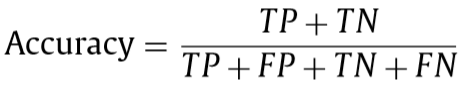
\includegraphics[width=0.5\textwidth]{imagenes/f2} 
	\end{figure}

	\item \textbf{Error rate}: Caso opuesto al accuracy, evaluando la proporción de los datos
	evaluados clasificados de forma incorrecta.
	\begin{figure}[H]
		\centering
		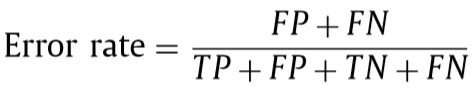
\includegraphics[width=0.5\textwidth]{imagenes/f3} 
	\end{figure}

	\item \textbf{Recall/sensitivity}: Medida de la proporción de TP que están correctamente clasificados.
	\begin{figure}[H]
		\centering
		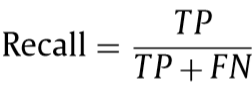
\includegraphics[width=0.3\textwidth]{imagenes/f4} 
	\end{figure}

	\item \textbf{Positive predictive value(PPV)/Precisión}: Proporción de las instancias del test que tienen una
	salida positiva y que además están bien clasificados.
	representa la probabilidad de que una prueba positiva 
	refleje la condición subyacente que se está probando.
	\begin{figure}[H]
		\centering
		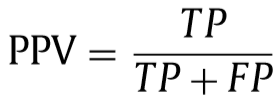
\includegraphics[width=0.3\textwidth]{imagenes/f5} 
	\end{figure}
\end{itemize}



\textbf{Clasificación multiclase}

Procedemos ahora a exponer algunas medidas de predicción aplicadas a los problemas de clasificación multiclase. Para ambas medidas hemos de tener en cuenta lo siguiente: n corresponde a la cantidad de observaciones en el conjunto de datos evaluados, $y'_i$ es la clase predicha para una instancia i e $y_i$ es la etiqueta de clase real (ambos representados como valores enteros basados en su posición en la escala ordinal).

\begin{itemize}
	\item \textbf{Mean Squared Error (MSE)}: Mide la media de los cuadrados de los errores. Al usar los cuadrados de $y_i$ e $y'_i$ se pondera con un peso mayor a los errores más grandes.
	\begin{figure}[H]
		\centering
		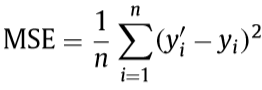
\includegraphics[width=0.4\textwidth]{imagenes/f6} 
	\end{figure}

	\item \textbf{Mean Absolute Error (MAE)}: Mide cómo de cerca se encuentran las predicciones de los valores reales de salida. MAE es una medida lineal, lo que significa que los errores son tratados con el mismo peso en la media.
	\begin{figure}[H]
		\centering
		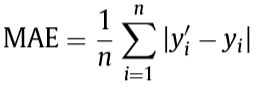
\includegraphics[width=0.4\textwidth]{imagenes/f7} 
	\end{figure}
\end{itemize}

Dados los conjuntos de datos de los que disponemos y el uso que la literatura recomienda hacer de las medidas de precisión sobre este tipo de conjuntos de datos, utilizaremos la medida\textbf{ Mean Absolute Error (MAE)} para la evaluación de la precisión de nuestros algoritmos, ya que los conjuntos que manejaremos son de clasificación multiclase.

\subsubsection{Medidas de monotonicidad}

Nuestro propósito con esta medida es evaluar la tasa de monotonicidad provista tanto por las predicciones obtenidas y el conjunto de datos original, como de la construcción del modelo.

Para ello tenemos en cuenta las siguientes consideraciones:
\begin{itemize}
	\item x es un ejemplo del conjunto de datos D.
	\item NClash(x) es la cantidad de ejemplos de D que no cumplen las restricciones de monotonicidad con respecto a x.
	\item n es el número de instancias en D.
	\item NMonot(x) es el número de ejemplos de D que sí que cumplen las restricciones de monotonicidad con respecto a x.
\end{itemize}

El \textbf{Índice de no-monotonicidad} se define como el número de choques (Nclash) dividido por el número de pares de ejemplos en el conjunto de datos:

\begin{figure}[H]
	\centering
	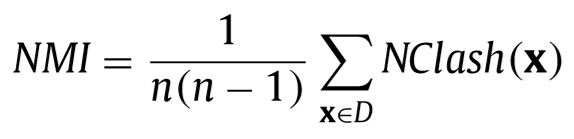
\includegraphics[width=0.5\textwidth]{imagenes/f8} 
\end{figure}

Y esta será la medida que utilicemos finalmente para la evaluación de la monotonicidad en nuestros algoritmos.

\section{Resultados}

\begin{table}[H]
	\begin{tabular}{|c|l|l|l|l|}
		\hline
		HOEFFDING TREE & ERA    & ESL    & LEV &  SWD \\ \hline
		MAE & 1.5110 & 0.6616 & 0.546                      & 0.6349                     \\ \hline
		NMI & 0.4028 & 0.2945 & 0.3338                     & 0.3227                     \\ \hline
	\end{tabular}
\caption{Resultados de accuracy y monotonicidad para los 4 data sets descritos mediante el uso de Hoeffding Tree algorithm.}
\end{table}

\section{Análisis}

\newpage











